\subsection{Kernel configuration}

\begin{frame}
  \frametitle{Kernel configuration}
  \begin{itemize}
  \item The kernel contains thousands of device drivers, filesystem
    drivers, network protocols and other configurable items
  \item Thousands of options are available, that are used to
    selectively compile parts of the kernel source code
  \item The kernel configuration is the process of defining the set of
    options with which you want your kernel to be compiled
  \item The set of options depends
    \begin{itemize}
    \item On the target architecture and on your hardware (for device drivers, etc.)
    \item On the capabilities you would like to give to your kernel
      (network capabilities, filesystems, real-time, etc.).
      Such generic options are available in all architectures.
    \end{itemize}
  \end{itemize}
\end{frame}

\begin{frame}
  \frametitle{Kernel configuration and build system}
  \begin{itemize}
  \item The kernel configuration and build system is based on multiple
    Makefiles
  \item One only interacts with the main \kfile{Makefile}, present at
    the {\bf top directory} of the kernel source tree
  \item Interaction takes place
    \begin{itemize}
    \item using the \code{make} tool, which parses the Makefile
    \item through various {\bf targets}, defining which action should
      be done (configuration, compilation, installation, etc.).
    \item Run \code{make help} to see all available targets.
    \end{itemize}
  \item Example
    \begin{itemize}
    \item \code{cd linux/}
    \item \code{make <target>}
    \end{itemize}
  \end{itemize}
\end{frame}

\begin{frame}
  \frametitle{Specifying the target architecture}
  First, specify the architecture for the kernel to build
  \begin{itemize}
  \item Set \code{ARCH} to the name of a directory under \kdir{arch}:\\
	\code{ARCH=arm} or \code{ARCH=arm64} or \code{ARCH=riscv}, etc
  \item By default, the kernel build system assumes that the
        kernel is configured and built for the host architecture
	(\code{x86} in our case, native kernel compiling)
  \item The kernel build system will use this setting to:
	\begin{itemize}
	\item Use the configuration options for the target
	      architecture.
	\item Compile the kernel with source code and headers
	      for the target architecture.
	\end{itemize}
  \end{itemize}
\end{frame}

\begin{frame}[fragile]
  \frametitle{Choosing a compiler}
  The compiler invoked by the kernel Makefile is \code{$(CROSS_COMPILE)gcc}
  \begin{itemize}
    \item Specifying the compiler is already needed at configuration
	  time, as some kernel configuration options depend on the
          capabilities of the compiler.
    \item When compiling natively
      \begin{itemize}
	 \item Leave \code{CROSS_COMPILE} undefined and the kernel
	    will be natively compiled for the host architecture
            using \code{gcc}.
      \end{itemize}
    \item When using a cross-compiler
      \begin{itemize}
      \item Specify the prefix of your cross-compiler executable, for
            example for \code{arm-linux-gnueabi-gcc}:\\
          \code{CROSS_COMPILE=arm-linux-gnueabi-}
      \end{itemize}
  \end{itemize}
  Set \code{LLVM} to \code{1} to compile your kernel with Clang.\\
  See our \href{https://bootlin.com/pub/conferences/2022/lee/opdenacker-llvm-tools-for-linux-kernel/opdenacker-llvm-tools-for-linux-kernel.pdf}
  {LLVM tools for the Linux kernel} presentation.
\end{frame}

\begin{frame}
  \frametitle{Specifying ARCH and CROSS\_COMPILE}
  There are actually two ways of defining \code{ARCH} and \code{CROSS_COMPILE}:
  \begin{itemize}
  \item Pass \code{ARCH} and \code{CROSS_COMPILE} on the \code{make}
    command line: \\
    \code{make ARCH=arm CROSS_COMPILE=arm-linux- ...} \\
    Drawback: it is easy to forget to pass these variables when
    you run any \code{make} command, causing your build and
    configuration to be screwed up.
  \item Define \code{ARCH} and \code{CROSS_COMPILE} as environment
    variables: \\
    \code{export ARCH=arm} \\
    \code{export CROSS_COMPILE=arm-linux-} \\
    Drawback: it only works inside the current shell or terminal. You
    could put these settings in a file that you source every time you
    start working on the project, see also the
    \url{https://direnv.net/} project.
  \end{itemize}
\end{frame}

\begin{frame}
  \frametitle{Initial configuration}
  Difficult to find which kernel configuration will work
  with your hardware and root filesystem. Start with one
  that works!
  \begin{itemize}
  \item Desktop or server case:
     \begin{itemize}
       \item Advisable to start with the configuration of your running
	  kernel:\\
	  \code{cp /boot/config-`uname -r` .config}
     \end{itemize}
   \item Embedded platform case:
     \begin{itemize}
       \item Default configurations stored in-tree as minimal
         configuration files (only listing settings that are different
         with the defaults) in \code{arch/<arch>/configs/}
       \item \code{make help} will list the available configurations for
         your platform
       \item To load a default configuration file, just run
         \code{make foo_defconfig} (will erase your current
         \code{.config}!)
         \begin{itemize}
           \item On ARM 32-bit, there is usually one default
             configuration per CPU family
           \item On ARM 64-bit, there is only one big default
             configuration to customize
         \end{itemize}
     \end{itemize}
  \end{itemize}
\end{frame}

\begin{frame}
  \frametitle{Create your own default configuration}
  \begin{itemize}
    \item Use a tool such as \code{make menuconfig} to make changes to
      the configuration
    \item Saving your changes will overwrite your \code{.config} (not
      tracked by Git)
    \item When happy with it, create your own default configuration file:
      \begin{itemize}
      \item Create a minimal configuration (non-default settings) file:\\
        \code{make savedefconfig}
      \item Save this default configuration in the right directory:\\
        \code{mv defconfig arch/<arch>/configs/myown_defconfig}
      \end{itemize}
    \item This way, you can share a reference configuration inside
      the kernel sources and other developers can now get the same
      \code{.config} as you by running \code{make myown_defconfig}
  \end{itemize}
\end{frame}

\begin{frame}
  \frametitle{Built-in or module?}
  \begin{itemize}
  \item The {\bf kernel image} is a {\bf single file}, resulting from
    the linking of all object files that correspond to features
    enabled in the configuration
    \begin{itemize}
    \item This is the file that gets loaded in memory by the
      bootloader
    \item All built-in features are therefore available as soon as the
      kernel starts, at a time where no filesystem exists
    \end{itemize}
  \item Some features (device drivers, filesystems, etc.) can however
    be compiled as {\bf modules}
    \begin{itemize}
    \item These are {\em plugins} that can be loaded/unloaded dynamically to
      add/remove features to the kernel
    \item Each {\bf module is stored as a separate file in the
        filesystem}, and therefore access to a filesystem is mandatory
      to use modules
    \item This is not possible in the early boot procedure of the
      kernel, because no filesystem is available
    \end{itemize}
  \end{itemize}
\end{frame}

\begin{frame}
  \frametitle{Kernel option types}
  There are different types of options, defined in \code{Kconfig} files:
  \begin{itemize}
  \item \code{bool} options, they are either
    \begin{itemize}
    \item {\em true} (to include the feature in the kernel) or
    \item {\em false} (to exclude the feature from the kernel)
    \end{itemize}
  \item \code{tristate} options, they are either
    \begin{itemize}
    \item {\em true} (to include the feature in the kernel image) or
    \item {\em module} (to include the feature as a kernel module) or
    \item {\em false} (to exclude the feature)
    \end{itemize}
  \item \code{int} options, to specify integer values
  \item \code{hex} options, to specify hexadecimal values\\
    Example: \kconfigval{CONFIG_PAGE_OFFSET}{0xC0000000}
  \item \code{string} options, to specify string values\\
    Example: \kconfigval{CONFIG_LOCALVERSION}{-no-network}\\
    Useful to distinguish between two kernels built from different options
  \end{itemize}
\end{frame}

\begin{frame}[fragile]
  \frametitle{Kernel option dependencies}
  Enabling a network driver requires the network stack to be enabled,
  therefore configuration symbols have two ways to express dependencies:
  \begin{columns}
    \column{0.4\textwidth}
    \begin{itemize}
    \item \code{depends on} dependency:
\scriptsize
\begin{verbatim}
config B
    depends on A
\end{verbatim}
      \begin{itemize}
      \item B is not visible until A is enabled
      \item Works well for dependency chains
      \end{itemize}
    \end{itemize}
    \column{0.6\textwidth}
    \begin{itemize}
    \item \code{select} dependency:
\scriptsize
\begin{verbatim}
config A
    select B
\end{verbatim}
      \begin{itemize}
      \item When A is enabled, B is enabled too (and cannot be disabled
        manually)
      \item Should preferably not select symbols with \code{depends on}
        dependencies
      \item Used to declare hardware features or select libraries
      \end{itemize}
    \end{itemize}
  \end{columns}
  \vfill
  \scriptsize
\begin{verbatim}
config SPI_ATH79
        tristate "Atheros AR71XX/AR724X/AR913X SPI controller driver"
        depends on ATH79 || COMPILE_TEST
        select SPI_BITBANG
        help
          This enables support for the SPI controller present on the
          Atheros AR71XX/AR724X/AR913X SoCs.
\end{verbatim}
\end{frame}

\begin{frame}[fragile]
  \frametitle{Kernel configuration details}
  \begin{columns}
    \column{0.65\textwidth}
    \begin{itemize}
    \item The configuration is stored in the \code{.config} file at the
      root of kernel sources
      \begin{itemize}
      \item Simple text file, \code{CONFIG_PARAM=value}
      \item Options are grouped by sections and are prefixed with
        \code{CONFIG_}
      \item Included by the top-level kernel Makefile
      \item Typically not edited by hand because of the dependencies
      \end{itemize}
    \end{itemize}
    \column{0.35\textwidth}
    \footnotesize
\begin{verbatim}
#
# CD-ROM/DVD Filesystems
#
CONFIG_ISO9660_FS=m
CONFIG_JOLIET=y
CONFIG_ZISOFS=y
CONFIG_UDF_FS=y
# end of CD-ROM/DVD Filesystems

#
# DOS/FAT/EXFAT/NT Filesystems
#
CONFIG_FAT_FS=y
CONFIG_MSDOS_FS=y
# CONFIG_VFAT_FS is not set
CONFIG_FAT_DEFAULT_CODEPAGE=437
# CONFIG_EXFAT_FS is not set
\end{verbatim}
  \end{columns}
\end{frame}

\begin{frame}
  \frametitle{xconfig}
  \begin{columns}
    \column{0.5\textwidth}
    \code{make xconfig}
    \begin{itemize}
    \item A graphical interface to configure the kernel.
    \item File browser: easy to load configuration files
    \item Search interface to look for parameters (\code{[Ctrl]} + \code{[f]})
    \item Required Debian/Ubuntu packages: \code{qt5-default}
          (\code{qtbase5-dev} on Ubuntu 22.04)
    \end{itemize}
    \column{0.5\textwidth}
    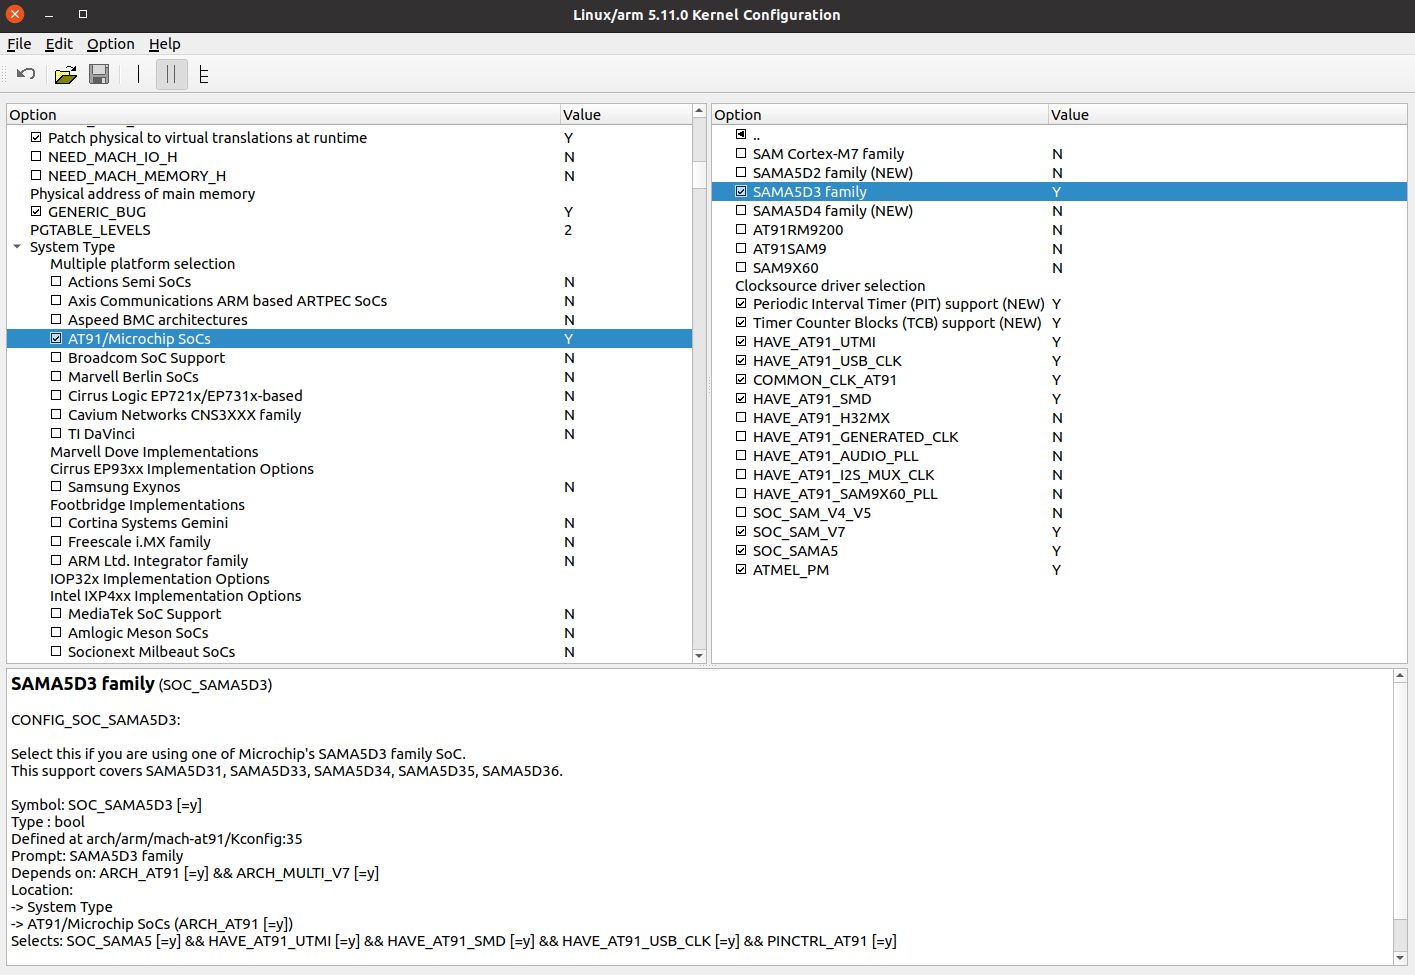
\includegraphics[width=\textwidth]{slides/sysdev-kernel-building/xconfig-screenshot.png}
  \end{columns}
\end{frame}

\begin{frame}
  \frametitle{menuconfig}
  \begin{columns}
    \column{0.5\textwidth}
    \code{make menuconfig}
    \begin{itemize}
      \item Useful when no graphics are available. Very efficient interface.
      \item Same interface found in other tools: BusyBox, Buildroot...
      \item Convenient number shortcuts to jump directly to search results.
      \item Required Debian/Ubuntu packages: \code{libncurses-dev}
    \end{itemize}
    \column{0.5\textwidth}
    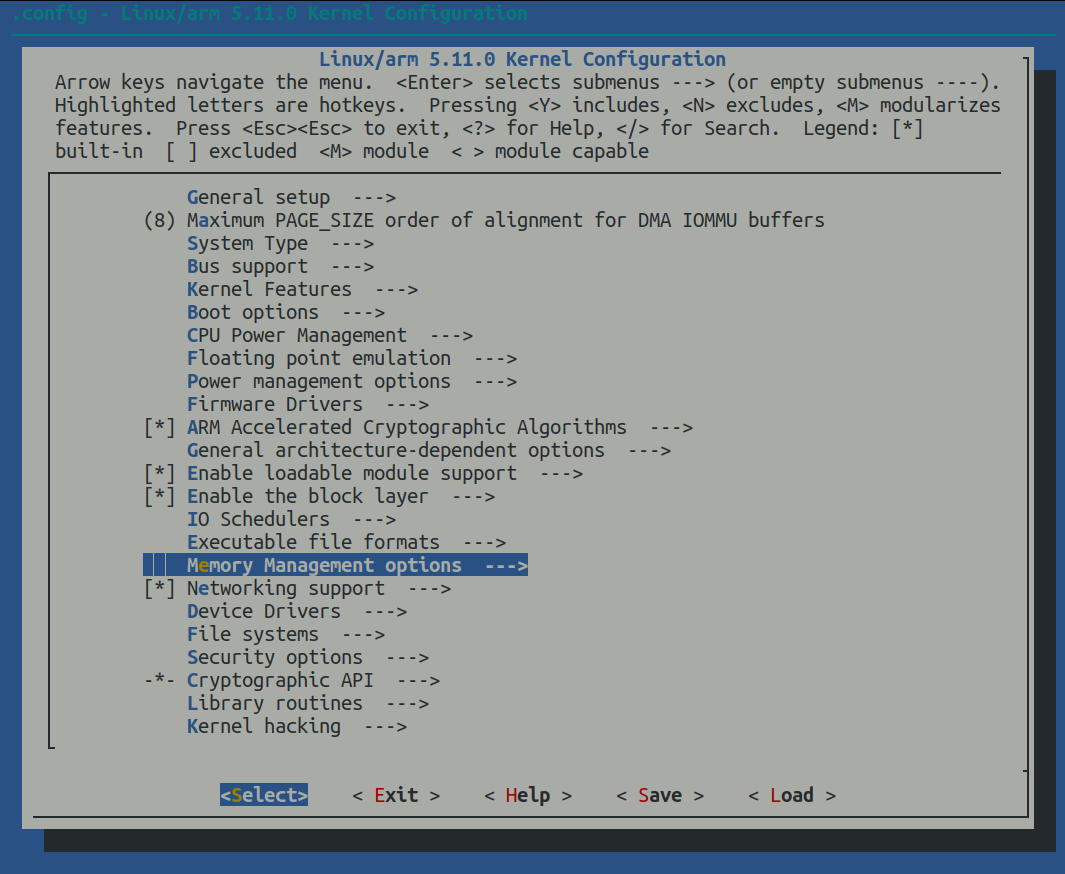
\includegraphics[width=\textwidth]{slides/sysdev-kernel-building/menuconfig-screenshot.png}
  \end{columns}
\end{frame}

\begin{frame}
  \frametitle{Kernel configuration options}
  You can switch from one tool to another, they all load/save the same
  \code{.config} file, and show the same set of options
  \begin{center}
    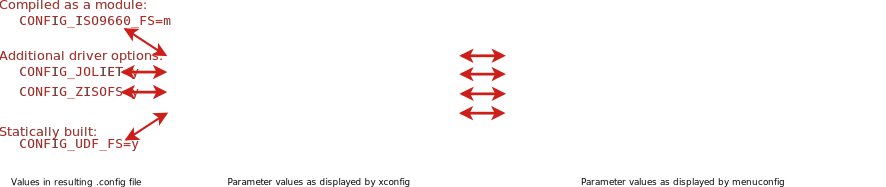
\includegraphics[width=\textwidth]{slides/sysdev-kernel-building/iso-example.pdf}
  \end{center}
\end{frame}

\begin{frame}
  \frametitle{make oldconfig}
  \code{make oldconfig}
  \begin{itemize}
  \item Useful to upgrade a \code{.config} file from an earlier kernel release
  \item Asks for values for new parameters.
  \item ... unlike \code{make menuconfig} and \code{make xconfig} which silently set
  default values for new parameters.
  \end{itemize}
  If you edit a \code{.config} file by hand, it's useful
  to run \code{make oldconfig} afterwards, to set values to new
  parameters that could have appeared because of dependency changes.
\end{frame}

\begin{frame}
  \frametitle{Undoing configuration changes}
  A frequent problem:
  \begin{itemize}
  \item After changing several kernel configuration settings, your
    kernel no longer works.
  \item If you don't remember all the changes you made,
    you can get back to your previous configuration:\\
    \code{$ cp .config.old .config}
  \item All the configuration tools keep this \code{.config.old} backup
    copy.
  \end{itemize}
\end{frame}

\subsection{Compiling and installing the kernel}

\begin{frame}[fragile]
  \frametitle{Kernel compilation}
  \begin{columns}
  \column{0.7\textwidth}
  \code{make}
  \begin{itemize}
    \item Only works from the top kernel source directory
    \item Should not be performed as a priviledged user
    \item Run several {\bf j}obs in parallel. Our advice: \code{ncpus * 2} to
      fully load the CPU and I/Os at all times.\\
          Example: \code{make -j 8}
    \item To {\bf re}compile faster (7x according to some benchmarks),\\
	  use the \code{ccache} compiler cache:\\
          \code{export CROSS_COMPILE="ccache arm-linux-"}
  \end{itemize}
  \column{0.3\textwidth}
    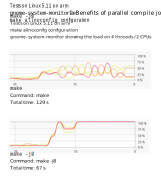
\includegraphics[width=\textwidth]{slides/sysdev-kernel-building/parallel-make-benefits.pdf}
  \end{columns}
\end{frame}

\begin{frame}
  \frametitle{Kernel compilation results}
  \begin{itemize}
    \item \code{arch/<arch>/boot/Image}, uncompressed kernel image that
      can be booted
    \item \code{arch/<arch>/boot/*Image*}, compressed kernel images that
      can also be booted
      \begin{itemize}
      \item \code{bzImage} for x86, \code{zImage} for ARM,
      \code{Image.gz} for RISC-V, \code{vmlinux.bin.gz} for ARC, etc.
      \end{itemize}
    \item \code{arch/<arch>/boot/dts/*.dtb}, compiled Device Tree Blobs
    \item All kernel modules, spread over the kernel source tree, as
      \code{.ko} ({\em Kernel Object}) files.
    \item \code{vmlinux}, a raw uncompressed kernel image in the ELF
      format, useful for debugging purposes but generally not used for
      booting purposes
  \end{itemize}
\end{frame}

\begin{frame}
  \frametitle{Kernel installation: native case}
  \begin{itemize}
  \item \code{sudo make install}
    \begin{itemize}
    \item Does the installation for the host system by default
    \end{itemize}
  \item Installs
    \begin{itemize}
    \item \code{/boot/vmlinuz-<version>} \\
      Compressed kernel image. Same as the one in
      \code{arch/<arch>/boot}
    \item \code{/boot/System.map-<version>}\\
      Stores kernel symbol addresses for debugging purposes
      (obsolete: such information is usually stored in the kernel itself)
    \item \code{/boot/config-<version>}\\
      Kernel configuration for this version
    \end{itemize}
  \item In GNU/Linux distributions, typically re-runs the bootloader configuration
    utility to make the new kernel available at the next boot.
  \end{itemize}
\end{frame}

\begin{frame}
  \frametitle{Kernel installation: embedded case}
  \begin{itemize}
  \item \code{make install} is rarely used in embedded development, as the
    kernel image is a single file, easy to handle.
  \item Another reason is that there is no standard way to deploy and
    use the kernel image.
  \item Therefore making the kernel image available to the target is
    usually manual or done through scripts in build systems.
  \item It is however possible to customize the \code{make install}
    behavior in \code{arch/<arch>/boot/install.sh}
  \end{itemize}
\end{frame}

\begin{frame}
  \frametitle{Module installation: native case}
  \begin{itemize}
  \item \code{sudo make modules_install}
    \begin{itemize}
    \item Does the installation for the host system by default, so
      needs to be run as root
    \end{itemize}
  \item Installs all modules in \code{/lib/modules/<version>/}
    \begin{itemize}
    \item \code{kernel/}\\
      Module \code{.ko} (Kernel Object) files, in the same directory
      structure as in the sources.
    \item \code{modules.alias}, \code{modules.alias.bin}\\
      Aliases for module loading utilities
      \ifthenelse{\equal{\training}{linux-kernel}}{, see next slide}{}
    \item \code{modules.dep}, \code{modules.dep.bin}\\
        Module dependencies. Kernel modules can depend on other modules,
        based on the symbols (functions and data structures) they use.
    \item \code{modules.symbols}, \code{modules.symbols.bin}\\
      Tells which module a given symbol belongs to (related to
      module dependencies).
    \item \code{modules.builtin}\\
      List of built-in modules of the kernel.
    \end{itemize}
  \end{itemize}
\end{frame}

\ifthenelse{\equal{\training}{linux-kernel}}{
\begin{frame}{Module alias: {\em modules.alias}}
  \begin{center}
    \includegraphics[width=\textwidth]{slides/kernel-hw-devices/module-alias-usage.pdf}
  \end{center}
\end{frame}
}{}

\begin{frame}
  \frametitle{Module installation: embedded case}
  \begin{itemize}
  \item In embedded development, you can't directly use
    \code{make modules_install} as it would install target modules
    in \code{/lib/modules} on the host!
  \item The \code{INSTALL_MOD_PATH} variable is needed to generate
    the module related files and install the modules in the target
    root filesystem instead of your host root filesystem (no need
    to be root):\\
    \code{make INSTALL_MOD_PATH=<dir>/ modules_install}
  \end{itemize}
\end{frame}

\begin{frame}[fragile]
  \frametitle{Kernel cleanup targets}
  \begin{columns}
    \column{0.8\textwidth}
    \small
    \begin{itemize}
    \item From \code{make help}:
    \begin{block}{}
    \begin{minted}[fontsize=\scriptsize]{console}
Cleaning targets:
  clean           - Remove most generated files but keep the config and
                    enough build support to build external modules
  mrproper        - Remove all generated files + config + various backup files
  distclean       - mrproper + remove editor backup and patch files
     \end{minted}
     \end{block}
    \item If you are in a git tree, remove all files not tracked (and
      ignored) by git:\\
      \code{git clean -fdx}
    \end{itemize}
    \column{0.2\textwidth}
    \includegraphics[width=0.9\textwidth]{slides/sysdev-kernel-building/kernel-mrproper.png}
  \end{columns}
\end{frame}

\begin{frame}
  \frametitle{Kernel building overview}
  \begin{center}
    \includegraphics[height=0.8\textheight]{slides/sysdev-kernel-building/kernel-building-overview.pdf}
  \end{center}
\end{frame}

\subsection{Booting the kernel}

\begin{frame}
  \frametitle{Hardware description}
  \begin{itemize}
  \item Many embedded architectures have a lot of non-discoverable
    hardware (serial, Ethernet, I2C, Nand flash, USB controllers...)
  \item This hardware needs to be described and passed to the Linux
    kernel.
  \item Using C code directly within the kernel is legacy, nowadays the
    bootloader/firmware is expected to provide this description when
    starting the kernel:
    \begin{itemize}
    \item On x86: using ACPI tables
    \item On most embedded devices: using an OpenFirmware Device Tree
      (DT)
    \end{itemize}
  \item This way, a kernel supporting different SoCs knows which
    SoC and device initialization hooks to run on the current board.
  \end{itemize}
\end{frame}
